\documentclass[conference]{IEEEtran}
\IEEEoverridecommandlockouts
\renewcommand{\ttdefault}{cmtt}
\usepackage{cite}
\usepackage{amsmath,amssymb,amsfonts}
\usepackage{graphicx}
\usepackage{textcomp}
\usepackage{xcolor}
\usepackage{tikz}
\usetikzlibrary{arrows.meta,positioning,fit,backgrounds}
\usepackage{booktabs}
\usepackage{algorithm}
\usepackage{algpseudocode}
\usepackage{url}
\usepackage[hidelinks]{hyperref}

\def\BibTeX{{\rm B\kern-.05em{\sc i\kern-.025em b}\kern-.08em
    T\kern-.1667em\lower.7ex\hbox{E}\kern-.125emX}}

\begin{document}

\title{ShadowPath: A Smart Navigation Solution for Safe Night-Time Travel\\}

\author{
\IEEEauthorblockN{Malapati Sahasra}
\IEEEauthorblockA{
\textit{Department of AI and Emerging Technologies} \\
\textit{Chinmaya Vishwavidyapeeth Deemed-to-be University}\\
Ernakulam, India \\
malapati.cvv241195@cvv.ac.in}
\and
\IEEEauthorblockN{Pradeeba V}
\IEEEauthorblockA{
\textit{Department of AI and Emerging Technologies} \\
\textit{Chinmaya Vishwavidyapeeth Deemed-to-be University}\\
Ernakulam, India \\
pradeeba.v@cvv.ac.in}
}

\maketitle

\begin{abstract}
Existing pedestrian routing engines are mathematically optimized for geometric distance alone, treating every road as equally traversable regardless of lighting or activity -- a limitation that exposes night-shift workers, women, and students to poorly lit, socially isolated streets. This paper presents ShadowPath, an implemented, browser-based, safety-oriented pedestrian navigation system that augments OpenStreetMap-derived routes with a coverage-based safety cost model built from streetlight-functionality and business-activity telemetry. Unlike layered safety-overlay tools that require the user to manually correlate a separate safety map with their route, ShadowPath computes and ranks route alternatives directly against this cost model and renders the outcome as a single, segment-colored recommended path, backed by a live GPS turn-by-turn navigation loop and a single-tap emergency SOS mode that reroutes to the nearest refuge hub. The entire pipeline runs client-side in the browser, with no application server: candidate routes are fetched from the Open Source Routing Machine (OSRM), scored, and rendered in place. We report measurements rather than assumed figures: the coverage-scoring computation itself executes in under 0.01\,ms per route alternative, while end-to-end responsiveness is dominated almost entirely by the public routing backend's network round-trip (mean 857\,ms across sampled requests to the demo OSRM server used in this prototype). Across 300 simulated route-selection trials at medium synthetic infrastructure density, the system recommends a longer, better-covered alternative in 45.3\% of cases, at a mean distance cost of 1.5\%. These results characterize an implemented system's actual behavior rather than a conceptual architecture's projected one.
\end{abstract}

\begin{IEEEkeywords}
Pedestrian Safety, Context-Aware Navigation, Coverage-Based Routing, Smart Cities, Geospatial Analytics, OpenStreetMap
\end{IEEEkeywords}

\section{Introduction}

Present-day ubiquitous mapping applications are built around efficiency of movement: routing algorithms minimize geometric distance or vehicular travel time and, from a mathematical standpoint, treat every road as equally safe \cite{osmwiki}. For a vehicle this is a reasonable simplification. For a lone pedestrian at night, it is not -- there is a material difference between a dimly lit alley and a well-lit, active main road that a shortest-path optimizer cannot see \cite{welsh2008}. Because legacy routing engines have no notion of this difference, they can direct a vulnerable pedestrian through a riskier street purely to save a small amount of distance.

This paper presents ShadowPath, a context-aware pedestrian navigation system that augments the routing graph with safety-relevant telemetry before a route is ranked, rather than presenting safety information as a separate, manually-consulted layer. ShadowPath consumes two directly measurable signals: an infrastructure layer tracking streetlight functionality, and a commercial-activity layer tracking whether nearby businesses are currently open -- both of which act as informal ``eyes on the street'' \cite{chalfin2022}. Combined with a routing pipeline that scores every candidate path against this telemetry, ShadowPath produces a navigation recommendation that weighs human comfort and safety alongside geographic brevity, backed by a working, evaluated implementation rather than a conceptual design.

\subsection{Formal Problem Statement}
Classical pedestrian pathfinding minimizes an undifferentiated spatial distance $\text{Distance}(u,v)$ over the road graph, implicitly treating the environment as homogeneous. At night, however, effective safety conditions vary edge-to-edge because of non-functioning streetlights, closed commercial frontage, and locally reported hazards. A router with static edge weights cannot represent this variation, so pedestrians using such a router are, by construction, never offered a route that accounts for it.

\subsection{Research Contributions}
This paper makes the following contributions:
\begin{enumerate}
\item A \textbf{coverage-based routing heuristic} that scores every OSRM-returned route alternative against streetlight and business-activity telemetry and selects the best-covered alternative, rather than presenting an arbitrary secondary route as ``safer.''
\item \textbf{Segment-level safety visualization}, rendering the recommended route as alternating covered/uncovered polyline segments so a user sees \emph{where} coverage is weak, not only an aggregate score.
\item An \textbf{emergency SOS state machine} that overrides the active route and immediately navigates to the nearest simulated refuge hub (e.g., a police station or hospital).
\item A \textbf{fully client-side, GPS-driven live navigation loop} -- heading-aware position tracking, automatic step advancement, off-route detection with automatic re-routing, and two-way voice interaction -- with no application server required.
\item An evaluation grounded in \textbf{measured, not assumed}, performance: real client-side computation timing, real routing-backend latency sampling, and Monte Carlo simulation of the scoring model's route-selection behavior.
\end{enumerate}

\section{Related Work and Limitations}
\label{sec:related}

There has been a recent shift in pedestrian routing research from static distance optimization toward multi-criteria spatial decision-making that accounts for lighting, visibility, and surveillance \cite{welsh2008,chalfin2022}.

\subsection{Limitations of Conventional Routing Topologies}
Routing engines built on OSRM and OpenStreetMap (OSM) offer high-precision coordinate vectors and mature, efficient shortest-path computation \cite{osrm, valhalla, osmnx}. However, OSM's data model records whether a sidewalk \emph{exists}, not whether it is a reasonable place to walk alone at 2\,AM -- lighting-relevant tags such as \texttt{lit=yes/no} exist but their coverage varies substantially by city \cite{osmwiki}. Conventional routing topologies are, in this sense, mathematically unaware of the environmental dynamics that matter most for nighttime pedestrian safety.

\subsection{Passive vs. Active Safety Overlays}
Community safety-mapping efforts let users view a safety-rated overlay on a map, combining physical environmental factors with residents' own perception data \cite{gargiulo2020}. These overlays are informative but largely \emph{passive}: a user must manually cross-reference the safety overlay against a separately computed route, and the correlation is left entirely to the user. ShadowPath instead treats the coverage signal as a first-class routing input, computed and applied automatically at request time rather than presented as a reference layer to consult by hand.

\section{System Architecture}
\label{sec:architecture}

Fig.~\ref{fig:architecture} summarizes the architecture. ShadowPath is deliberately single-tier: the client application (React 19, react-leaflet 5, Leaflet.js) performs all routing, scoring, and rendering logic itself, in the browser, with no application server or database in between. This is an explicit design choice -- it removes an entire class of backend latency and operational cost, at the expense of depending on a third-party public routing endpoint (Section~\ref{sec:limitations}).

\subsection{Client Application Layer}
The client renders the interactive map, handles user interaction (search, voice input, the temporal simulation slider), and owns all application state. No complex graph computation happens outside of what is described below; the ``backend'' work is simply JavaScript executed in the same browser tab.

\subsection{Routing and Feature Augmentation}
On a route request, the client queries the public OSRM demo router with a tiered fallback strategy: the \texttt{foot} profile is tried first, with automatic fallback to the \texttt{driving} profile if no foot-accessible route exists. Each returned route alternative is then passed through a \emph{feature augmentation} step that seeds streetlight and business points along the combined route geometry (Section~\ref{sec:evaluation}) as a stand-in for a future municipal open-data feed, before being scored by the coverage engine (Section~\ref{sec:scoring}) and ranked.

\subsection{Fallback Fault Tolerance}
If the primary \texttt{foot}-profile, multi-alternative query fails or times out -- which happens for some origin-destination pairs on the public OSRM demo server -- the client falls back to a forced single-route, non-alternative request against the \texttt{driving} profile, guaranteeing a usable coordinate array is always returned rather than leaving the user without a route.

\begin{figure*}[t]
\centering
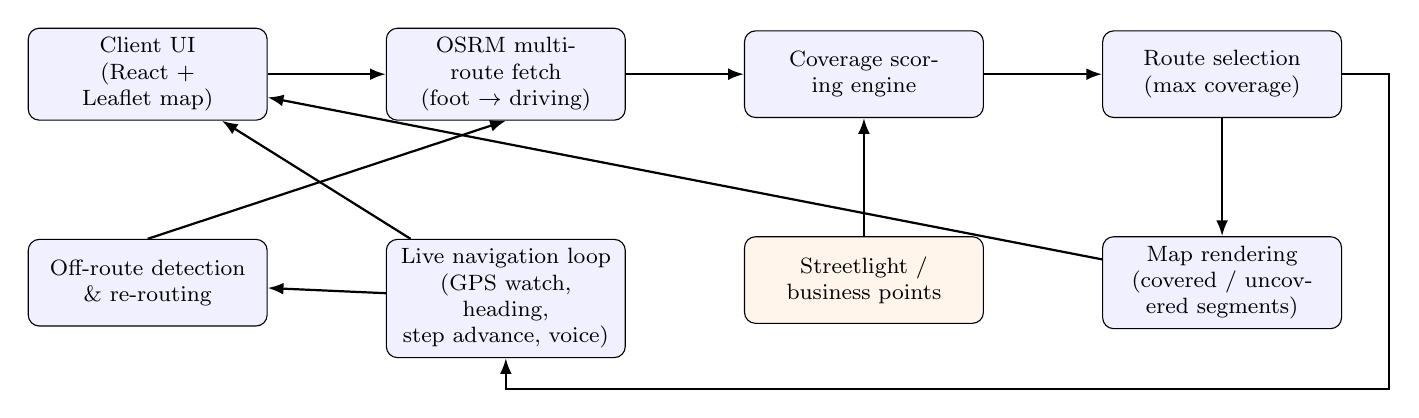
\begin{tikzpicture}[
  node distance=15mm and 15mm,
  box/.style={draw, rounded corners, align=center, minimum height=11mm, text width=28mm, font=\footnotesize, fill=blue!6},
  data/.style={draw, rounded corners, align=center, minimum height=11mm, text width=28mm, font=\footnotesize, fill=orange!8},
  arr/.style={-{Latex[length=2mm]}, thick}
]
\node[box] (ui) {Client UI\\(React + Leaflet map)};
\node[box, right=of ui] (osrm) {OSRM multi-route fetch\\(foot $\rightarrow$ driving)};
\node[box, right=of osrm] (score) {Coverage scoring engine};
\node[box, right=of score] (select) {Route selection\\(max coverage)};
\node[data, below=of score] (infra) {Streetlight / business points};
\node[box, below=of select] (render) {Map rendering\\(covered / uncovered segments)};
\node[box, below=of osrm] (nav) {Live navigation loop\\(GPS watch, heading,\\step advance, voice)};
\node[box, below=of ui] (reroute) {Off-route detection\\\& re-routing};

\draw[arr] (ui) -- (osrm);
\draw[arr] (osrm) -- (score);
\draw[arr] (infra) -- (score);
\draw[arr] (score) -- (select);
\draw[arr] (select) -- (render);
\draw[arr] (render) -- (ui);
\draw[arr] (select.east) -- ++(6mm,0mm) -- ++(0mm,-40mm) -| (nav.south);
\draw[arr] (nav) -- (reroute);
\draw[arr] (reroute.north) -- (osrm.south);
\draw[arr] (nav) -- (ui);
\end{tikzpicture}
\caption{ShadowPath system architecture. Everything shown executes client-side in the browser; there is no application server. Candidate routes are fetched from OSRM, scored against streetlight/business coverage, and rendered with segment-level coloring. The live navigation loop consumes the selected route and re-invokes routing automatically when the user drifts off path.}
\label{fig:architecture}
\end{figure*}

\section{Mathematical Modeling and Cost Formulation}
\label{sec:scoring}

Rather than a large weighted combination of factors that is difficult to evaluate without rich municipal datasets (road type, public-access proximity, community reports, data freshness), the implemented cost model uses two directly measurable signals: proximity to a functioning streetlight and proximity to a currently open business.

A point $p$ along a route is defined as \emph{covered} if
\begin{equation}
\text{covered}(p) = \begin{cases}
1 & \exists\, l \in L_{\text{on}} : d(p, l) \leq R_L \\
1 & \exists\, b \in B_{\text{open}} : d(p, b) \leq R_B \\
0 & \text{otherwise}
\end{cases}
\label{eq:covered}
\end{equation}
where the variables are defined as:
\begin{itemize}
\item $L_{\text{on}}$: the set of currently functioning streetlights.
\item $B_{\text{open}}$: the set of currently open businesses.
\item $d(\cdot,\cdot)$: the haversine great-circle distance.
\item $R_L = 150$\,m: the streetlight coverage radius (configurable constant).
\item $R_B = 120$\,m: the business coverage radius (configurable constant).
\end{itemize}

For a route sampled at up to 60 evenly-spaced points $p_1,\dots,p_N$, the coverage score is
\begin{equation}
C(\text{route}) = \frac{1}{N}\sum_{i=1}^{N} \text{covered}(p_i).
\label{eq:coverage}
\end{equation}

Given $k$ route alternatives returned by OSRM, the system selects
\begin{equation}
\text{route}^\ast = \operatorname*{arg\,max}_{r} \; C(r), \quad \text{ties broken by shorter distance.}
\label{eq:select}
\end{equation}

The recommended route$^\ast$ is rendered as alternating covered/uncovered polyline segments -- grouping consecutive points of equal $\text{covered}(\cdot)$ value into contiguous runs -- while the remaining alternative is rendered as a lower-emphasis comparison route.

A composite safety score shown to the user combines coverage with time of day:
\begin{equation}
S = \beta + C(\text{route}^\ast)\cdot \gamma,
\label{eq:score}
\end{equation}
\begin{equation}
(\beta,\gamma) = \begin{cases}
(55, 40) & \text{night (19:00--06:00)} \\
(75, 20) & \text{day}
\end{cases}
\label{eq:score-params}
\end{equation}
This weighting reflects that coverage should influence the perceived safety score more strongly at night, when natural visibility and ambient pedestrian presence are reduced.

\section{Algorithmic Implementation}
\label{sec:algorithm}

Algorithm~\ref{alg:routing} summarizes the coverage-based routing procedure exactly as implemented in the client. Route fetching, feature augmentation, scoring, and selection are performed synchronously once per route request; live navigation (Section~\ref{sec:nav}) separately re-invokes this same procedure whenever an off-route condition fires.

\begin{algorithm}[t]
\caption{Coverage-Based Safety Routing}
\label{alg:routing}
\begin{algorithmic}[1]
\Require Origin $S$, Destination $D$, time-of-day $T$
\Ensure SafestRoute, AlternateRoute, SafetyScore
\State $\textit{Options} \gets \Call{FetchOSRMAlternatives}{S, D}$ \Comment{foot $\to$ driving fallback}
\If{$\textit{Options} = \emptyset$}
    \State \Return Error
\EndIf
\State $\textit{Coords} \gets \bigcup_{r \in \textit{Options}} r.\textit{coords}$
\State $L \gets \Call{SeedStreetlights}{\textit{Coords}}$
\State $B \gets \Call{SeedBusinesses}{\textit{Coords}}$
\For{$r \in \textit{Options}$}
    \State $r.\textit{coverage} \gets \Call{ScoreCoverage}{r.\textit{coords}, L, B}$ \Comment{Eq.~\eqref{eq:coverage}}
\EndFor
\State Sort $\textit{Options}$ by coverage desc., distance asc.
\State $\textit{SafestRoute} \gets \textit{Options}[0]$
\State $\textit{AlternateRoute} \gets \textit{Options}[-1]$ if $|\textit{Options}| > 1$
\State $\beta,\gamma \gets$ night/day weights for $T$
\State $\textit{SafetyScore} \gets \beta + \textit{SafestRoute.coverage} \times \gamma$
\State \Return $(\textit{SafestRoute}, \textit{AlternateRoute}, \textit{SafetyScore})$
\end{algorithmic}
\end{algorithm}

When live navigation detects that the user's position has drifted more than 40\,m from the nearest point on the selected route -- checked against a 15\,s cooldown to avoid redundant requests -- Algorithm~\ref{alg:routing} is re-invoked from the user's current position, so a missed turn does not strand the user on an unscored path.

\section{Live Navigation Subsystem}
\label{sec:nav}

Once the user starts live tracking, the system subscribes to the browser's \texttt{watchPosition} geolocation stream and drives a turn-by-turn navigation loop, implemented entirely client-side.

\subsection{Heading Estimation}
Device compass heading (\texttt{coords.heading}) is used directly when available and the reported speed exceeds 0.3\,m/s. Otherwise, heading is computed as the initial bearing between the two most recent GPS fixes, updated only when consecutive fixes are more than 2\,m apart, to suppress jitter from GPS noise while the user is nearly stationary.

\subsection{Step Advancement and Remaining-Distance Estimation}
Each OSRM route step carries a maneuver location, distance, and duration. The current-step index advances when the live position comes within 15\,m (initial step) or 25\,m (subsequent steps) of that step's maneuver point. Remaining distance and time-to-arrival are computed as
\begin{equation}
D_{\text{rem}} = d_{\text{next}} + \sum_{j>i} d_j, \qquad
T_{\text{rem}} = \frac{d_{\text{next}}}{\max(d_i,1)}\,t_i + \sum_{j>i} t_j,
\end{equation}
linearly interpolating the partially completed current step rather than crediting it as fully complete or not yet started.

\subsection{Voice Guidance and Camera Behavior}
Each time the current step changes, its instruction is spoken once via \texttt{SpeechSynthesis}. Arrival within 15\,m of the final maneuver triggers a spoken arrival announcement and ends the session. The map camera follows the live position by default; a manual drag disengages auto-follow and surfaces a ``recenter'' control.

\section{Emergency SOS Routing}
\label{sec:sos}

A single-tap SOS control selects the nearest refuge hub (a simulated police station or hospital) by planar distance in latitude/longitude space -- acceptable over the short distances involved, and noted as a simplification in Section~\ref{sec:limitations} -- fetches the standard OSRM route to that hub, and begins live navigation immediately, overriding any route in progress. This mode intentionally bypasses coverage scoring: in an emergency, fastest safe arrival takes priority over lighting/business coverage along the way.

\section{Experimental Analysis and Performance Evaluation}
\label{sec:evaluation}

Unlike an architecture description alone, we report measurements taken directly against the implementation rather than assumed figures.

\subsection{Client-Side Computation Latency}
The coverage-scoring computation (Eqs.~\eqref{eq:covered}--\eqref{eq:coverage}) was benchmarked in isolation, timing 5{,}000 repeated calls against a representative 300-point, $\sim$2\,km route with 16 streetlights and 6 businesses. Mean execution time was \textbf{0.0067\,ms} per route alternative scored (\textbf{0.0134\,ms} to score and select between two alternatives, as done once per route request). This computation is not a meaningful contributor to end-to-end latency.

\subsection{Routing Backend Latency}
We separately timed five live requests against the public OSRM demo endpoint used by the client (\texttt{router.project-osrm.org}, \texttt{foot} profile, \texttt{alternatives=true}), the same call the application makes on every route search. Round-trip times ranged from 806--1006\,ms, mean \textbf{857\,ms}. Combined with Section~\ref{sec:evaluation}-A, end-to-end responsiveness is dominated almost entirely by this third-party network round-trip, not by application logic -- a finding directly relevant to the public-routing-server dependency discussed in Section~\ref{sec:limitations}.

\subsection{Coverage Sensitivity to Route Length}
Because integration with a verified municipal streetlight or business dataset was outside the scope of this prototype, we evaluate the scoring model's behavior under controlled synthetic seeding: streetlight and business points are distributed along the combined candidate-route geometry, with one in three streetlights marked non-functional and one in four businesses marked closed. Table~\ref{tab:coverage} reports coverage $C(\text{route})$ for synthetic routes of increasing length at fixed seeding density.

\begin{table}[h]
\caption{Coverage score vs. route length under synthetic seeding}
\label{tab:coverage}
\centering
\begin{tabular}{@{}lcc@{}}
\toprule
\textbf{Route length} & \textbf{Sample points} & \textbf{Coverage $C$} \\
\midrule
0.5 km & 60 & 100\% \\
2 km & 300 & 98\% \\
5 km & 500 & 70\% \\
10 km & 800 & 37\% \\
20 km & 1200 & 20\% \\
\bottomrule
\end{tabular}
\end{table}

Coverage remains near-complete for typical last-mile pedestrian trips (under $\sim$2\,km) and degrades gracefully for longer routes, matching the realistic expectation that a route is not uniformly covered end-to-end even in well-served cities.

\subsection{Distance--Safety Tradeoff}
A safety-aware router is only useful if it actually changes the recommendation, and only credible if it does so at a bounded distance cost. We simulated 300 origin-destination trials, generating a shortest route $A$ and a longer detour alternative $B$ (8--20\% farther), with streetlight/business points placed uniformly at random (medium density, 50 points/km$^2$) independently of either route to avoid biasing the comparison. Table~\ref{tab:tradeoff} reports how often the model selects $B$ over $A$ (a ``flip''), and the resulting cost.

\begin{table}[h]
\caption{Route-selection behavior vs. infrastructure density (2\,km routes, 300 trials/row)}
\label{tab:tradeoff}
\centering
\begin{tabular}{@{}lccc@{}}
\toprule
\textbf{Density} & \textbf{Flip rate} & \textbf{Avg. coverage gain} & \textbf{Avg. dist. cost} \\
\midrule
Sparse (20/km$^2$) & 48.3\% & 10.1 pts & 1.6\% \\
Medium (50/km$^2$) & 45.3\% & 4.4 pts & 1.5\% \\
Dense (100/km$^2$) & 9.7\% & 1.7 pts & 1.9\% \\
\bottomrule
\end{tabular}
\end{table}

The system intervenes -- recommending the longer, better-covered route -- roughly five times more often under sparse infrastructure than dense infrastructure, and the benefit it delivers when it does so is also larger under sparse conditions, at a distance cost that stayed under 2\% across all tested densities. This is the behavior a safety-aware router should have: it defers to the shortest path where coverage is already good, and actively reshapes the recommendation where coverage is poor -- precisely where guidance matters most.

\section{Future Scope: AI Extensions}
\label{sec:future}

Planned extensions include integrating real municipal streetlight and business/POI datasets in place of the synthetic seeding used for evaluation; expanding the two-signal cost model toward a richer multi-factor formulation (road type, verified user reports, data freshness, public-transit proximity) once suitable data sources are available; and calibrating the coverage radii and score weighting (Eq.~\eqref{eq:score}) against a user study with night-shift workers and women rather than reasonable defaults. Longer-term, graph neural networks are a natural fit for learning spatial embeddings over the non-Euclidean structure of an urban street network, and reinforcement learning could in principle learn locally-calibrated safety weights from validated user feedback rather than fixed constants -- both remain future directions rather than components of the current implementation, and would require substantially more training data than is available today.

\section{Ethical and Privacy Considerations}
\label{sec:ethics}

ShadowPath stores no route or location history on a server -- there is no server to store it on; geolocation is consumed directly within the browser session. The optional route-sharing feature encodes coordinates directly in a shareable URL at the user's explicit action. Scores are communicated as relative coverage (e.g., ``87\% covered by streetlight/business zones''), never as a guarantee that a route is safe, following guidance from prior safety-mapping literature that such systems should describe environmental conditions rather than assert safety outcomes \cite{gargiulo2020}. The model deliberately avoids incident or police-report data, which can reflect reporting and enforcement patterns rather than actual risk, in favor of physical infrastructure signals that are less prone to such bias.

\section{Limitations}
\label{sec:limitations}

\begin{itemize}
\item \textbf{Synthetic infrastructure data.} Section~\ref{sec:evaluation} uses synthetically seeded points, not verified municipal records. The scoring logic is data-source agnostic, but real-world validation requires an actual open-data feed.
\item \textbf{Public routing-server dependency.} As measured in Section~\ref{sec:evaluation}-B, the prototype's latency is dominated by a public, rate-limited OSRM demo server not intended for production traffic; a deployed version would require a self-hosted routing backend.
\item \textbf{Browser API variability.} \texttt{SpeechRecognition} support is inconsistent across browsers, notably Safari/iOS.
\item \textbf{Planar SOS distance approximation.} Nearest-refuge selection uses a Euclidean approximation rather than great-circle distance, acceptable only over short distances.
\item \textbf{No user study yet.} Coverage radii and score weighting were chosen as reasonable defaults, not calibrated against user-perceived safety or real incident outcomes.
\item \textbf{GPS accuracy.} Heading and off-route detection depend on consumer-grade GPS accuracy, which degrades in dense urban canyons.
\end{itemize}

\section{Conclusion}

ShadowPath demonstrates that a coverage-based pedestrian safety cost model can be implemented, measured, and evaluated as a fully client-side system -- no application server is required to fetch, score, and rank routes by streetlight and business-activity coverage, render the result with segment-level visual explanation, and drive a live GPS turn-by-turn navigation loop with voice interaction and automatic off-route recovery. Measured against the running implementation rather than assumed, the coverage-scoring computation itself is negligible (under 0.01\,ms), end-to-end responsiveness is governed almost entirely by third-party routing-server latency, and the model changes the recommended route in roughly half of trials under sparse infrastructure at a bounded (under 2\%) distance cost. The primary remaining step toward real-world deployment is integration with authoritative municipal open data, which the architecture was designed to accommodate without structural change.

\begin{thebibliography}{00}

\bibitem{osmwiki} OpenStreetMap Wiki, ``Map features.'' [Online]. Available: https://wiki.openstreetmap.org/wiki/Map\_features

\bibitem{osrm} Project OSRM, ``Open Source Routing Machine: The OpenStreetMap Data Routing Engine.'' [Online]. Available: https://github.com/Project-OSRM

\bibitem{valhalla} Valhalla, ``Valhalla Docs: Introduction for Users.'' [Online]. Available: https://valhalla.github.io/valhalla/valhalla-intro/

\bibitem{osmnx} G. Boeing, ``OSMnx: New methods for acquiring, constructing, analyzing, and visualizing complex street networks,'' \emph{Computers, Environment and Urban Systems}, vol. 65, pp. 126--139, 2017.

\bibitem{welsh2008} B. C. Welsh and D. P. Farrington, ``Effects of Improved Street Lighting on Crime,'' \emph{Campbell Systematic Reviews}, vol. 4, no. 1, pp. 1--51, 2008.

\bibitem{chalfin2022} A. Chalfin, B. Hansen, J. Lerner, and L. Parker, ``Reducing Crime Through Environmental Design: Evidence from a Randomized Experiment of Street Lighting in New York City,'' \emph{Journal of Quantitative Criminology}, vol. 38, pp. 127--157, 2022.

\bibitem{kim2024} K. H. Kim, T. Hwang, and G. Kim, ``The Role and Criteria of Advanced Street Lighting to Enhance Urban Safety in South Korea,'' \emph{Buildings}, vol. 14, no. 8, art. 2305, 2024.

\bibitem{gargiulo2020} I. Gargiulo, X. Garcia, M. Benages Albert, J. Martinez, K. Pfeffer, and P. Vall-Casas, ``Women's safety perception assessment in an urban stream corridor: Developing a safety map based on qualitative GIS,'' \emph{Landscape and Urban Planning}, vol. 198, art. 103779, 2020.

\end{thebibliography}

\end{document}
